%----------------------------------------------------------------------------------------
%	PACKAGES AND THEMES
%----------------------------------------------------------------------------------------

\documentclass{beamer}

\usepackage{Style/style}

%----------------------------------------------------------------------------------------
%	TITLE PAGE
%----------------------------------------------------------------------------------------

% The short title appears at the bottom of every slide, the full title is only on the title page
\title[]{Animal Shelter Outcomes\\
		 Data Mining Kaggle Competition} 

\author[PoliKagglers]
{%
	\textbf{PoliKagglers}\\	
	E. Bertino, A. Donizetti, P. Necchi, A. Negrini, M. Toschi
}
		 
\institute[Polimi] % Your institution as it will appear on the bottom of every slide, may be shorthand to save space
{%
Politecnico di Milano%\\ % Your institution for the title page
%\medskip
%\textit{john@smith.com} % Your email address
}
\date{\today}

\begin{document}

\begin{frame}[plain]
     \begin{tikzpicture}[remember picture,overlay]
         \node[at=(current page.center)] {
             \includegraphics[width=\paperwidth]{Images/cover}
         };
     \end{tikzpicture}
\end{frame}

%------------------------------------------------------------------------------
% Indice 
%------------------------------------------------------------------------------

\begin{frame}
\frametitle{Plan} % Table of contents slide, comment this block out to remove it
\tableofcontents % Throughout your presentation, if you choose to use \section{} and \subsection{} commands, these will automatically be printed on this slide as an overview of your presentation
\end{frame}

%------------------------------------------------------------------------------
% Corpo della presentazione 
%------------------------------------------------------------------------------

\section{Introduction}

\begin{frame}[c]{Introduction}
	\begin{block}{TODO}
		\begin{itemize}
			\item Put kaggle logo
			\item Describe animal shelter competition (animal photo?)
		\end{itemize}
	\end{block}
\end{frame}

\section{Data Exploration}

\begin{frame}[c]{Animal Status}
	\vspace{-0.5cm}
	\begin{center}
		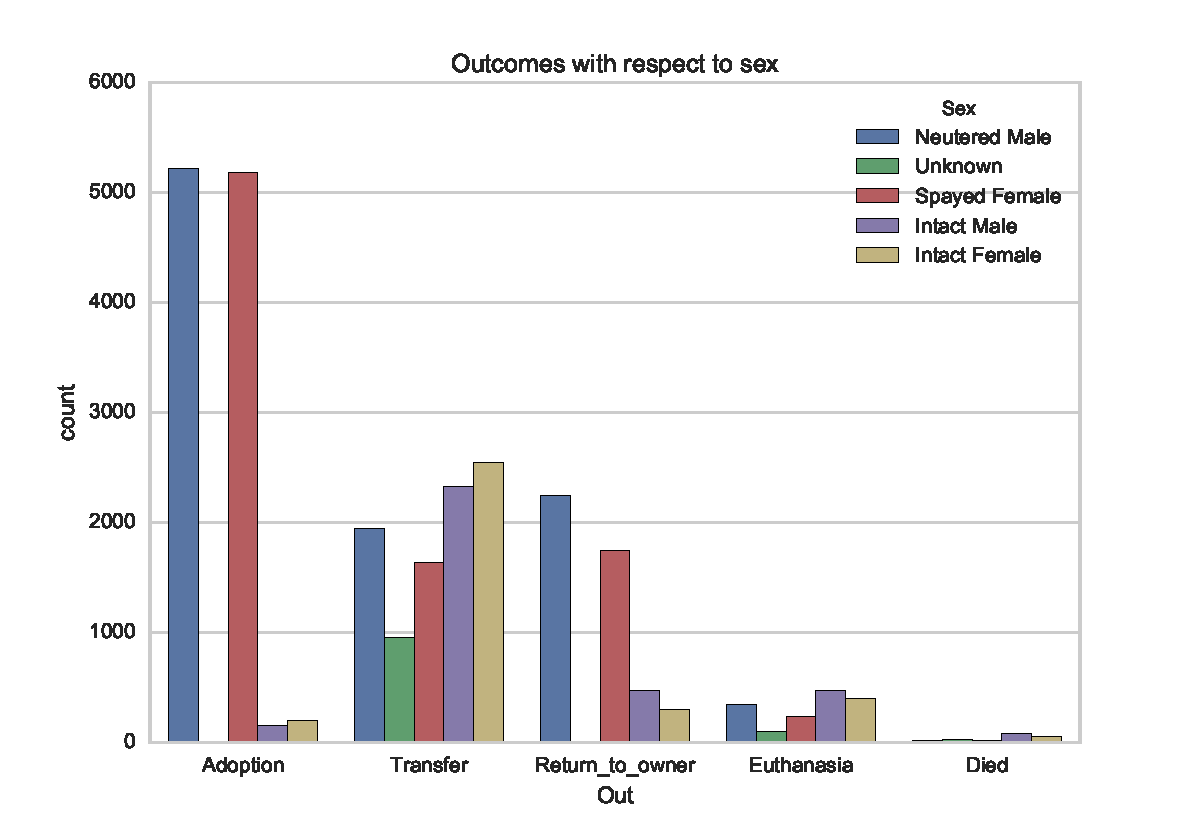
\includegraphics[width=1\linewidth]{Images/figure_2}
	\end{center}
\end{frame}

\begin{frame}[c]{Hourly Patterns}
	\vspace{-0.5cm}
	\begin{center}
		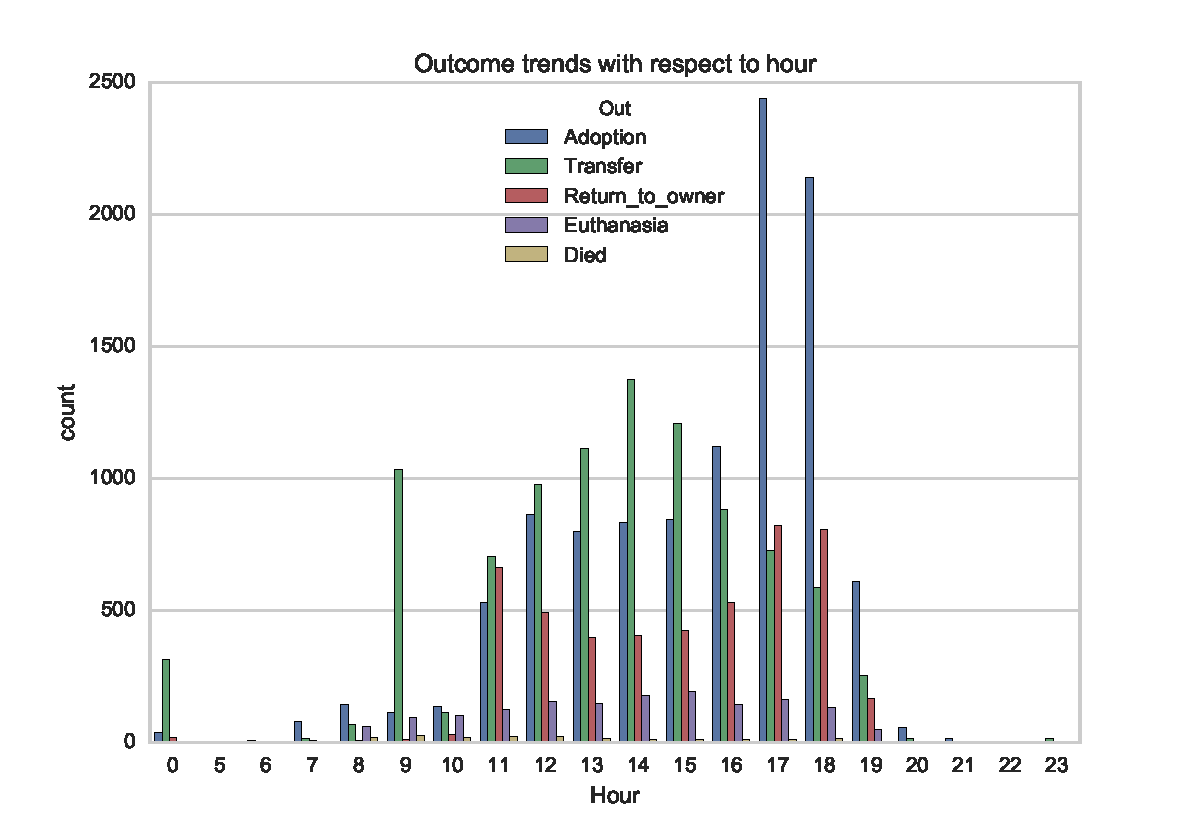
\includegraphics[width=1\linewidth]{Images/figure_4}
	\end{center}
\end{frame}

\section{Dealing With Leaks}

\begin{frame}[c]{Leak}
	\begin{block}{Two sources of leak}
		\begin{itemize}
			\item Data is gathered at outcome time
				\begin{itemize}
					\item Animal status is a strong outcome predictor
				\end{itemize}
			\item Training set and test set overlap in time
				\begin{itemize}
					\item Outcome time provides very rich information
				\end{itemize}
		\end{itemize}
	\end{block}
\end{frame}

\section{Feature Engineering}

\begin{frame}[t]{Features}	
	\begin{table}[t]
	\centering
	\begin{tabular}{@{}lllll@{}}
	\toprule
	Original Variable & Type        & Variables obtained & Type        & Leak \\ \midrule
	Name             & String      & Length of name     & Numerical   & No   \\
	Date and time    & Datetime    & Year               & Numerical   & Yes  \\
					 &             & Season             & Numerical   & No   \\
					 &			   & Holidays			& Categorical & No \\
					 &             & Month              & Numerical   & No   \\
					 &             & Day of week        & Numerical   & No   \\
					 &             & Day                & Numerical   & Yes  \\
					 &             & Day of year        & Numerical   & Yes  \\
					 &             & Hour               & Numerical   & Yes  \\
					 &             & Minute             & Numerical   & Yes  \\
					 &             & Minute of day      & Numerical   & Yes  \\
					 &             & Outcomes clusters  & Numerical   & Yes  \\
	Animal type      & Categorical & Animal Type        & Categorical & No   \\
	Sex upon outcome & Categorical & Gender             & Categorical & No   \\
					 &             & Status             & Categorical & Yes  \\
	Age upon outcome & Ordinal     & Age in days        & Numerical   & No   \\
			&	   & GroupAges		& Categorical & No\\
	Breed            & Categorical & Breed Groups       & Categorical & No   \\
					 &             & Mix and multibreed & Categorical & No   \\
					 &             & Dangerous          & Categorical & No   \\
	Color            & Categorical & Number of colors   & Numerical   & No   \\
					 &             & Color groups       & Categorical & No   \\
					 &             & Pattern            & Categorical & No   \\ \bottomrule
	\end{tabular}
	\end{table}
\end{frame}

\begin{frame}[t]{Outcomes Temporal Clustering}
	TODO: diagramma?
\end{frame}


\section{Classification Pipeline}

\subsection{Classification Methods}
	
\begin{frame}[t]{Classifiers and Software}
	
	\begin{alertblock}{Random Forests and Xgboost}
		\begin{itemize}
			\item High flexibility and ability to handle ``mixed'' data-types.
			\item Typically work well out-of-the-box
			\item Xgboost has proven extremely successful in past Kaggle
				competitions. 
			\item Quite easy to fine-tune. 
		\end{itemize}
	\end{alertblock}
	\begin{block}{May the python be with you}
		\begin{itemize}
			\item Pandas
			\item Scikit-Learn 
			\item Xgboost
		\end{itemize}
	\end{block}
\end{frame}

\subsection{Model Validation}

\begin{frame}[c]{Model Validation and Parameter Tuning}
	\begin{itemize}
		\item Extracted a stratified holdout set from the training set
		\item Used early stopping to avoid overfitting in xgboost classifier
		\item Evaluated several performance metrics on the holdout set
		\item Tuned xgboost parameters using CV-based grid search
		\item Bagged several xgboost classifiers to reduce variance
	\end{itemize}
\end{frame}

\subsection{Results}

\begin{frame}[c]{Project Milestones}
	% TODO: use resizebox
	\begin{table}[t]
		\centering
		\begin{tabular}{@{}lll@{}}
		\toprule
		Description                                      & Score   & Leaderboard \\ \midrule
		Bagged xgboost classifier with no leak           & 0.91586 & 667         \\
		Added animal status                              & 0.81768 & 454         \\
		Added day, hour and minute information           & 0.69699 & 21          \\
		Added outcome clusters                           & 0.64574 & 4           \\
		Tuned xgboost parameters by grid search          & 0.62799 & 4           \\
		Hierarchical xgboost \& random forest classifier & 0.62713 & 4           \\ \bottomrule
		\end{tabular}
	\end{table}

\end{frame}

\section{Conclusions}

\begin{frame}[t]{Conclusions and Further Developments}
	\begin{block}{Conclusions}
		\begin{itemize}
			\item<+-> ``Leak'' variables have a huge predictive power 
			\item<+-> Exploiting temporal clusters of outcomes, we reached the
				3rd position worldwide.
			\item<+-> Fine-tuning of the xgboost parameters yields large
				improvements in classification accuracy
		\end{itemize}
	\end{block}
	\pause
	\begin{block}{Further Developments}
		\begin{itemize}
			\item<+-> Design features to separate adoptions and return to owners
			\item<+-> Combine different classifiers able to learn different aspects 
		\end{itemize}
	\end{block}
\end{frame}




%------------------------------------------------------------------------------
% Appendice
%------------------------------------------------------------------------------
\appendix
\backupbegin

\begin{frame}
\frametitle{\refname}
\nocite{*}
\bibliography{Bibliography/bibliography}
\end{frame}

\backupend

\end{document}
